\documentclass{standalone}
\usepackage{tikz}
\usetikzlibrary{patterns, positioning}

\begin{document}
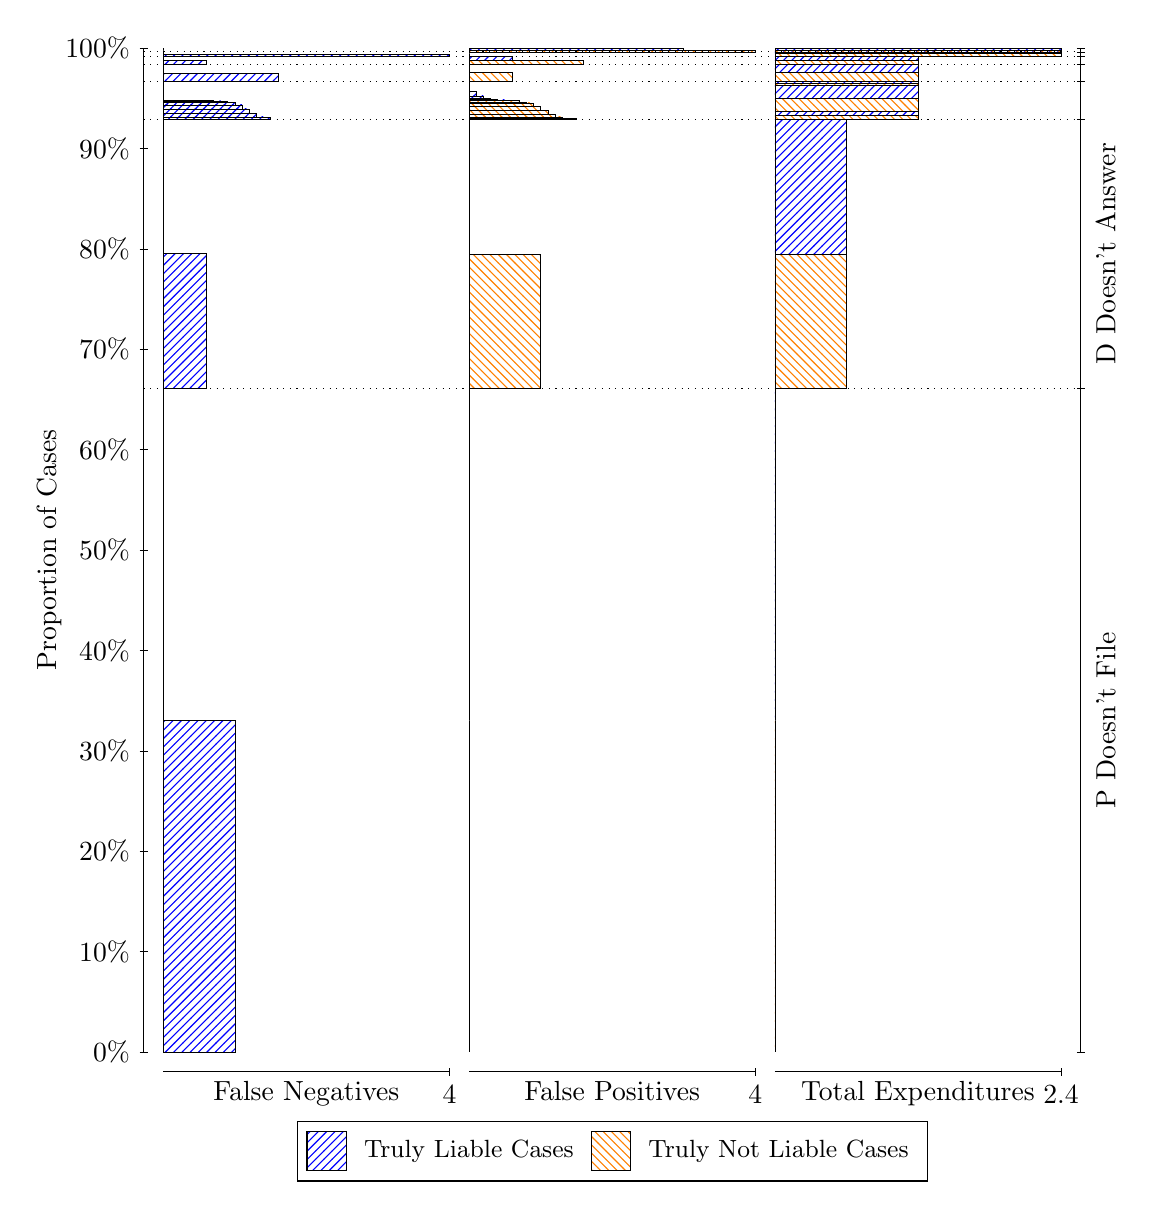
\begin{tikzpicture}
\draw[black, very thin] (1.5,1.75) -- (1.5,14.5);
\node[rotate=90, anchor=center] at (0.3, 8.125) {Proportion of Cases};
\draw[black, very thin] (1.45,1.75) -- (1.55,1.75);
\node[anchor=east] at (1.45, 1.75) {0\%};
\draw[black, very thin] (1.45,3.025) -- (1.55,3.025);
\node[anchor=east] at (1.45, 3.025) {10\%};
\draw[black, very thin] (1.45,4.3) -- (1.55,4.3);
\node[anchor=east] at (1.45, 4.3) {20\%};
\draw[black, very thin] (1.45,5.575) -- (1.55,5.575);
\node[anchor=east] at (1.45, 5.575) {30\%};
\draw[black, very thin] (1.45,6.85) -- (1.55,6.85);
\node[anchor=east] at (1.45, 6.85) {40\%};
\draw[black, very thin] (1.45,8.125) -- (1.55,8.125);
\node[anchor=east] at (1.45, 8.125) {50\%};
\draw[black, very thin] (1.45,9.4) -- (1.55,9.4);
\node[anchor=east] at (1.45, 9.4) {60\%};
\draw[black, very thin] (1.45,10.675) -- (1.55,10.675);
\node[anchor=east] at (1.45, 10.675) {70\%};
\draw[black, very thin] (1.45,11.95) -- (1.55,11.95);
\node[anchor=east] at (1.45, 11.95) {80\%};
\draw[black, very thin] (1.45,13.225) -- (1.55,13.225);
\node[anchor=east] at (1.45, 13.225) {90\%};
\draw[black, very thin] (1.45,14.5) -- (1.55,14.5);
\node[anchor=east] at (1.45, 14.5) {100\%};

\draw[black, very thin] (13.4,1.75) -- (13.4,14.5);
\draw[black, very thin] (13.35,1.75) -- (13.45,1.75);
\node[anchor=west] at (13.35, 1.75) {};
\draw[black, very thin] (13.35,10.173) -- (13.45,10.173);
\node[anchor=west] at (13.35, 10.173) {};
\draw[black, very thin] (13.35,13.595) -- (13.45,13.595);
\node[anchor=west] at (13.35, 13.595) {};
\draw[black, very thin] (13.35,14.077) -- (13.45,14.077);
\node[anchor=west] at (13.35, 14.077) {};
\draw[black, very thin] (13.35,14.295) -- (13.45,14.295);
\node[anchor=west] at (13.35, 14.295) {};
\draw[black, very thin] (13.35,14.394) -- (13.45,14.394);
\node[anchor=west] at (13.35, 14.394) {};
\draw[black, very thin] (13.35,14.452) -- (13.45,14.452);
\node[anchor=west] at (13.35, 14.452) {};
\draw[black, very thin] (13.35,14.5) -- (13.45,14.5);
\node[anchor=west] at (13.35, 14.5) {};

\draw[black, very thin, pattern color=blue, pattern=north east lines] (1.75,1.75) rectangle (2.6583,5.9614);
\draw[black, very thin, pattern color=orange, pattern=north west lines] (1.75,5.9614) rectangle (1.75,10.173);
\draw[black, very thin, pattern color=blue, pattern=north east lines] (1.75,10.173) rectangle (2.295,11.888);
\draw[black, very thin, pattern color=orange, pattern=north west lines] (1.75,11.888) rectangle (1.75,13.595);
\draw[black, very thin, pattern color=blue, pattern=north east lines] (1.75,13.595) rectangle (3.1125,13.615);
\draw[black, very thin, pattern color=blue, pattern=north east lines] (1.75,13.615) rectangle (3.0217,13.625);
\draw[black, very thin, pattern color=blue, pattern=north east lines] (1.75,13.625) rectangle (2.9308,13.67);
\draw[black, very thin, pattern color=blue, pattern=north east lines] (1.75,13.67) rectangle (2.84,13.727);
\draw[black, very thin, pattern color=blue, pattern=north east lines] (1.75,13.727) rectangle (2.7492,13.779);
\draw[black, very thin, pattern color=blue, pattern=north east lines] (1.75,13.779) rectangle (2.6583,13.807);
\draw[black, very thin, pattern color=blue, pattern=north east lines] (1.75,13.807) rectangle (2.5675,13.824);
\draw[black, very thin, pattern color=blue, pattern=north east lines] (1.75,13.824) rectangle (2.4767,13.83);
\draw[black, very thin, pattern color=blue, pattern=north east lines] (1.75,13.83) rectangle (2.3858,13.837);
\draw[black, very thin, pattern color=orange, pattern=north west lines] (1.75,13.837) rectangle (1.75,14.077);
\draw[black, very thin, pattern color=blue, pattern=north east lines] (1.75,14.077) rectangle (3.2033,14.182);
\draw[black, very thin, pattern color=orange, pattern=north west lines] (1.75,14.182) rectangle (1.75,14.295);
\draw[black, very thin, pattern color=blue, pattern=north east lines] (1.75,14.295) rectangle (2.295,14.346);
\draw[black, very thin, pattern color=orange, pattern=north west lines] (1.75,14.346) rectangle (1.75,14.394);
\draw[black, very thin, pattern color=blue, pattern=north east lines] (1.75,14.394) rectangle (5.3833,14.416);
\draw[black, very thin, pattern color=orange, pattern=north west lines] (1.75,14.416) rectangle (1.75,14.452);
\draw[black, very thin, pattern color=orange, pattern=north west lines] (1.75,14.452) rectangle (1.75,14.471);
\draw[black, very thin, pattern color=blue, pattern=north east lines] (1.75,14.471) rectangle (1.75,14.5);
\draw[black, very thin, pattern color=orange, pattern=north west lines] (5.6333,1.75) rectangle (5.6333,5.9614);
\draw[black, very thin, pattern color=blue, pattern=north east lines] (5.6333,5.9614) rectangle (5.6333,10.173);
\draw[black, very thin, pattern color=orange, pattern=north west lines] (5.6333,10.173) rectangle (6.5417,11.88);
\draw[black, very thin, pattern color=blue, pattern=north east lines] (5.6333,11.88) rectangle (5.6333,13.595);
\draw[black, very thin, pattern color=orange, pattern=north west lines] (5.6333,13.595) rectangle (6.9958,13.602);
\draw[black, very thin, pattern color=orange, pattern=north west lines] (5.6333,13.602) rectangle (6.905,13.609);
\draw[black, very thin, pattern color=orange, pattern=north west lines] (5.6333,13.609) rectangle (6.8142,13.626);
\draw[black, very thin, pattern color=orange, pattern=north west lines] (5.6333,13.626) rectangle (6.7233,13.655);
\draw[black, very thin, pattern color=orange, pattern=north west lines] (5.6333,13.655) rectangle (6.6325,13.706);
\draw[black, very thin, pattern color=orange, pattern=north west lines] (5.6333,13.706) rectangle (6.5417,13.761);
\draw[black, very thin, pattern color=orange, pattern=north west lines] (5.6333,13.761) rectangle (6.4508,13.804);
\draw[black, very thin, pattern color=orange, pattern=north west lines] (5.6333,13.804) rectangle (6.36,13.813);
\draw[black, very thin, pattern color=orange, pattern=north west lines] (5.6333,13.813) rectangle (6.2692,13.835);
\draw[black, very thin, pattern color=blue, pattern=north east lines] (5.6333,13.835) rectangle (6.0875,13.842);
\draw[black, very thin, pattern color=blue, pattern=north east lines] (5.6333,13.842) rectangle (5.9967,13.849);
\draw[black, very thin, pattern color=blue, pattern=north east lines] (5.6333,13.849) rectangle (5.9058,13.865);
\draw[black, very thin, pattern color=blue, pattern=north east lines] (5.6333,13.865) rectangle (5.815,13.893);
\draw[black, very thin, pattern color=blue, pattern=north east lines] (5.6333,13.893) rectangle (5.7242,13.945);
\draw[black, very thin, pattern color=blue, pattern=north east lines] (5.6333,13.945) rectangle (5.6333,14.077);
\draw[black, very thin, pattern color=orange, pattern=north west lines] (5.6333,14.077) rectangle (6.1783,14.19);
\draw[black, very thin, pattern color=blue, pattern=north east lines] (5.6333,14.19) rectangle (5.6333,14.295);
\draw[black, very thin, pattern color=orange, pattern=north west lines] (5.6333,14.295) rectangle (7.0867,14.343);
\draw[black, very thin, pattern color=blue, pattern=north east lines] (5.6333,14.343) rectangle (6.1783,14.394);
\draw[black, very thin, pattern color=orange, pattern=north west lines] (5.6333,14.394) rectangle (5.6333,14.43);
\draw[black, very thin, pattern color=blue, pattern=north east lines] (5.6333,14.43) rectangle (5.6333,14.452);
\draw[black, very thin, pattern color=orange, pattern=north west lines] (5.6333,14.452) rectangle (9.2667,14.471);
\draw[black, very thin, pattern color=blue, pattern=north east lines] (5.6333,14.471) rectangle (8.3583,14.5);
\draw[black, very thin, pattern color=orange, pattern=north west lines] (9.5167,1.75) rectangle (9.5167,5.9614);
\draw[black, very thin, pattern color=blue, pattern=north east lines] (9.5167,5.9614) rectangle (9.5167,10.173);
\draw[black, very thin, pattern color=orange, pattern=north west lines] (9.5167,10.173) rectangle (10.425,11.88);
\draw[black, very thin, pattern color=blue, pattern=north east lines] (9.5167,11.88) rectangle (10.425,13.595);
\draw[black, very thin, pattern color=orange, pattern=north west lines] (9.5167,13.595) rectangle (11.333,13.647);
\draw[black, very thin, pattern color=blue, pattern=north east lines] (9.5167,13.647) rectangle (11.333,13.7);
\draw[black, very thin, pattern color=orange, pattern=north west lines] (9.5167,13.7) rectangle (11.333,13.863);
\draw[black, very thin, pattern color=blue, pattern=north east lines] (9.5167,13.863) rectangle (11.333,14.029);
\draw[black, very thin, pattern color=orange, pattern=north west lines] (9.5167,14.029) rectangle (11.333,14.053);
\draw[black, very thin, pattern color=blue, pattern=north east lines] (9.5167,14.053) rectangle (11.333,14.077);
\draw[black, very thin, pattern color=orange, pattern=north west lines] (9.5167,14.077) rectangle (11.333,14.19);
\draw[black, very thin, pattern color=blue, pattern=north east lines] (9.5167,14.19) rectangle (11.333,14.295);
\draw[black, very thin, pattern color=orange, pattern=north west lines] (9.5167,14.295) rectangle (11.333,14.343);
\draw[black, very thin, pattern color=blue, pattern=north east lines] (9.5167,14.343) rectangle (11.333,14.394);
\draw[black, very thin, pattern color=orange, pattern=north west lines] (9.5167,14.394) rectangle (13.15,14.43);
\draw[black, very thin, pattern color=blue, pattern=north east lines] (9.5167,14.43) rectangle (13.15,14.452);
\draw[black, very thin, pattern color=orange, pattern=north west lines] (9.5167,14.452) rectangle (13.15,14.471);
\draw[black, very thin, pattern color=blue, pattern=north east lines] (9.5167,14.471) rectangle (13.15,14.5);
\draw[black, dotted] (1.5,10.173) -- (13.4,10.173);
\draw[black, dotted] (1.5,13.595) -- (13.4,13.595);
\draw[black, dotted] (1.5,14.077) -- (13.4,14.077);
\draw[black, dotted] (1.5,14.295) -- (13.4,14.295);
\draw[black, dotted] (1.5,14.394) -- (13.4,14.394);
\draw[black, dotted] (1.5,14.452) -- (13.4,14.452);
\draw[black, very thin] (1.75,1.5) -- (5.3833,1.5);
\node[anchor=north] at (3.5667, 1.5) {False Negatives};
\draw[black, very thin] (5.3833,1.45) -- (5.3833,1.55);
\node[anchor=north] at (5.3833, 1.45) {4};

\draw[black, very thin] (5.6333,1.5) -- (9.2667,1.5);
\node[anchor=north] at (7.45, 1.5) {False Positives};
\draw[black, very thin] (9.2667,1.45) -- (9.2667,1.55);
\node[anchor=north] at (9.2667, 1.45) {4};

\draw[black, very thin] (9.5167,1.5) -- (13.15,1.5);
\node[anchor=north] at (11.333, 1.5) {Total Expenditures};
\draw[black, very thin] (13.15,1.45) -- (13.15,1.55);
\node[anchor=north] at (13.15, 1.45) {2.4};

\node[black, centered, rotate=90] at (13.72, 5.9614) {P Doesn't File};
\node[black, centered, rotate=90] at (13.72, 11.884) {D Doesn't Answer};






\draw (7.449999999999999,1.5) node[draw=none] (baseCoordinate) {};
\begin{scope}[align=center]
        \matrix[scale=0.5, draw=black, below=0.5cm of baseCoordinate, nodes={draw}, column sep=0.1cm]{
            \node[rectangle, draw, minimum width=0.5cm, minimum height=0.5cm, pattern=north east lines, pattern color=blue] {}; &
            \node[draw=none, font=\small] (B) {Truly Liable Cases}; &
            \node[rectangle, draw, minimum width=0.5cm, minimum height=0.5cm, pattern=north west lines, pattern color=orange] {}; &
            \node[draw=none, font=\small] (B) {Truly Not Liable Cases}; \\
            };
\end{scope}

\end{tikzpicture}
\end{document}